\documentclass[8pt, a4paper]{article}
\usepackage{multicol}
\usepackage{listings}
\usepackage{geometry}
\usepackage{graphicx}
\usepackage{caption}
\usepackage{xstring}

\geometry{margin=0.3cm}
\graphicspath{{img}}

\pagenumbering{gobble}
\date{}

\lstdefinestyle{customstyle}{
    basicstyle=\ttfamily\scriptsize,
    breakatwhitespace=true,         
    breakautoindent=true,
    breaklines=true,                 
    captionpos=t,                    
    keepspaces=false,                 
    showspaces=false,                
    showstringspaces=false,
    showtabs=false,                  
    frame=none,
    stepnumber=1,                                           % the step between two line-numbers. If it's 1 each line will be numbered
    tabsize=2
}

\renewcommand\lstlistingname{}
\DeclareCaptionFormat{listing}{}
\captionsetup[lstlisting]{labelformat=empty}

\newcommand{\lstinputwithcaption}[2]{%
  \lstinputlisting[caption={\texttt{#2}}]{#1}%
}
\newcommand{\codeListing}[6] {

  \begin{multicols}{2}
    \lstinputwithcaption{#1}{#2}

    \columnbreak

    \lstinputwithcaption{#3}{#4}

  \end{multicols}

  \begin{center}
    \includegraphics[scale=#5]{#6}
  \end{center}

}

\lstset{style=customstyle}

\begin{document}

NAMA: Radinal Shidiq Saragih

KELAS: IF C 2023

NPM: 5520123104

\begin{enumerate}
  \item Buatlah contoh program Java untuk DataInputStream dan DataOutputStream untuk menghitung pembelanjaan

  \begin{multicols}{2}

    \lstinputwithcaption{./code/src/pembelanjaan/Main.java}{Main.java}
    \lstinputwithcaption{./code/src/pembelanjaan/Transaksi.java}{Transaksi.java}
  \end{multicols}

      \begin{center}
        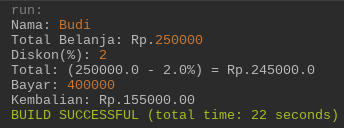
\includegraphics[scale=0.6]{OUTPUT1.png}
      \end{center}

  \item Jelaskan perbedaan penggunaan class Scanner dan class BufferReader
    dalam Java! Buatlah contoh program yang menunjukkan perbedaan tersebut

  \begin{itemize}
    \item Scanner Dapat membaca berbagai tipe data (int, double, String, dll.) secara langsung.
    \item BufferedReader Hanya membaca input sebagai String, perlu konversi manual ke tipe data lain.
    \item BufferedReader Lebih cepat karena tidak melakukan parsing otomatis, cocok untuk input besar.
    \item Scanner Lebih lambat karena melakukan parsing tipe data secara otomatis.
    \item Scanner Mudah digunakan untuk input dengan berbagai tipe data karena menyediakan metode seperti nextInt() dan nextLine().
    \item BufferedReader Lebih kompleks karena membutuhkan konversi tipe data secara manual.
    \item BufferedReader Memerlukan penanganan IOException.
    \item Scanner Tidak memerlukan IOException di konstruktornya, namun tetap perlu menangani InputMismatchException saat parsing
  \end{itemize}

    \lstinputwithcaption{./code/src/perbedaan\_input/Main.java}{Main.java}
    
      \begin{center}
        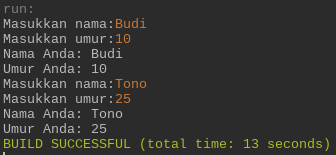
\includegraphics[scale=0.6]{OUTPUT2.png}
      \end{center}


  \item Buatlah program untuk menghitung gaya sentripetal

    \lstinputwithcaption{./code/src/gaya\_sentripal/Main.java}{Main.java}

      \begin{center}
        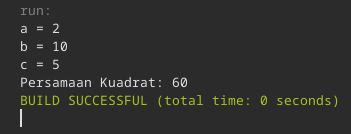
\includegraphics[scale=0.6]{OUTPUT3.png}
      \end{center}

  \item Ibu sisca pergi ke mini market untuk membeli 2 jenis buah, buah yang
    pertama dibeli adalah buah mangga sebanyak 70 pcs, dan membeli buah jambu
    untuk di berikan kepada 4 tetangganya, masing-masing tetangganya diberi
    30 pcs buah jambu, setelah ditimbang ternyata ada 15 pcs buah mangga yang
    busuk dan harus dikembalikan. Selesaikanlah menggunakan program Java untuk
    menghitung total buah yang dibeli menggunakan BufferedReader dan
    InputStreamReader

    \lstinputwithcaption{./code/src/total\_buah/Main.java}{Main.java}

    \begin{center}
      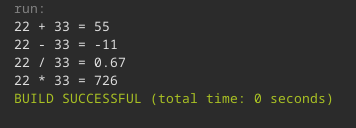
\includegraphics[scale=0.6]{OUTPUT4.png}
    \end{center}

  \item Buatlah program Java untuk menghitung selisih waktu dari waktu pertama
    dan kedua 

    \codeListing
      {./code/src/selisih\_waktu/Waktu.java}{Waktu.java}
      {./code/src/selisih\_waktu/Main.java}{Main.java}
      {0.6}{OUTPUT5.png}

  \item Buatlah program untuk menghitung berapa waktu yang diperlukan untuk
    menyelesaikan percetakan novel, mesin cetak yang digunakan memiliki
    kecepatan 1 lembar/detik. Keluaran dari program yaitu hari, jam,
    menit, dan detik. Dengan memberikan inputan terlebih dahulu 
    seperti banyaknya novel yang akan dicetak dan tebalnya lembar
    per novel tersebut.

    \lstinputwithcaption{./code/src/waktu\_cetak/Main.java}{Main.java}

      \begin{center}
        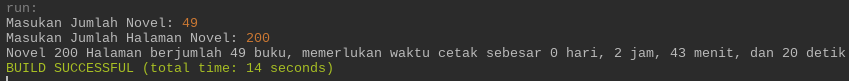
\includegraphics[scale=0.6]{OUTPUT6.png}
      \end{center}

\end{enumerate}

\end{document}
